

\section{The development cycle}
\index{program development!cycle|(}



We can see programs being developed in a cycle. 
\begin{center}
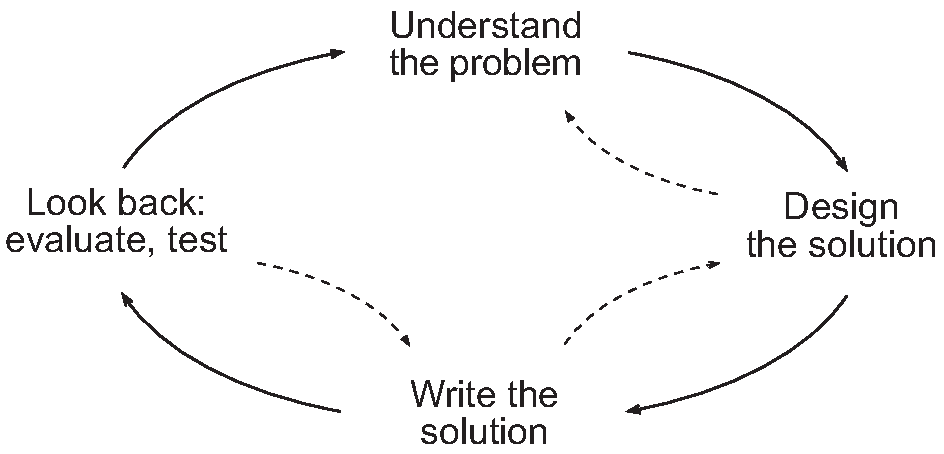
\includegraphics{Pictures/designCycle.pdf}
\end{center}
First, we have to
\textbf{understand the programming problem} that we are trying to solve -- we
spent some time talking about this in Chapter \ref{writingProgs}. Once
we have done this we can try to \textbf{plan} or \textbf{design}\index{design!role of} how we
might approach the problem, using all the resources of the programming
language, its libraries and also the programs that we have already
written. Again in Chapter \ref{writingProgs} we argued that we can make
considerable progress at this stage before we actually start to \textbf{write
programs}, which is the next step in the cycle.

Once the program is complete we can \textbf{reflect}
or\index{reflection}\index{looking back}
\textbf{look back} and see how well we have
achieved our goal: we might test the program -- as outlined in Chapter \ref{writingProgs}
-- or we might at this stage try to prove various properties of the programs we have written.
We can also at this point look back at the original problem -- was that 
in fact what the user wanted to solve, or in the light of seeing a running
program does the user want to change the specification of the problem? 

This clockwise cycle of stages is a simplified model of the way that
software is built in practice, from small exercise programs to large-scale
industrial projects. Even for the sort of programs we are writing here,
\textbf{reflecting} on what we are doing is a very important activity, and this
is emphasized by the dotted arrows in the cycle diagram. 
\begin{itemize}
\item
As we design a
program, we get further insight about how it should be specified: we
might find there are cases missed, or questions unanswered by the
specification -- we need to go back to the specifier and sort these out
before we can move on.
\item 
Also at the design stage we might think of competing approaches to
solving the problem: we need to think about which will be the better,
and maybe we will find that we have to change our approach if our first choice
proves to be unworkable.
\item
In writing the program we may well see how the design could be improved.
An example we have seen already concerns the index created in Section
\ref{indexExam}: in that case we kept hold of short words right until
the last stage in the composition while we could have got rid of them at
a much earlier stage: at the point where the lines were split into
words, say.
\end{itemize}
Especially when we are learning to program it is very good to get into
the habit of criticizing our own and other people's programs. Sometimes,
indeed, we find that after we have written a program we have gained  so much
deeper an understanding of the problem and the ways that we might solve
it that we throw away our first solution and rewrite it from scratch in order to
clean it up and to reflect our better understanding.

It is hard to give general advice about how to write programs, but some
of the most important ideas are contained in  the table in Figure
\ref{devCycle1}. The advice contained there is
strongly influenced by Polya's approach to problem solving in
mathematics, and his {\em How To Solve It\/} \cite{HowToSolveIt} contains a wealth of
suggestions about how to go about looking for solutions to problems,
many of which carry over to programming examples. The suggestion of
error logging is an integral part of  Humphrey's {\em Personal Software
Process\/} \cite{psp}.

In the next section we illustrate some of the points in the development
cycle using Haskell programming examples.


\index{program development!cycle|)}
\newcommand{\itemstart}{\smallskip\noindent$\circ$\hspace*{3mm}}
\begin{figure}

{\sc \textbf{Understanding the problem}}\hspace*{1mm}\hrulefill\\

First we need to understand the problem we are trying to solve. 

\itemstart
What are the inputs and outputs to the problem? Are there any special
conditions on the inputs or outputs?

\itemstart
Looking at examples can help to clarify the problem.

\itemstart
Can the problem be solved? Is the specification complete, or are there
aspects which need clarification?

\itemstart
If there are different possible ways of making sense of it, try to find
out from the specifier what was intended.

\itemstart
Does the problem itself have a structure? Is it made up of a number of
parts which could be solved separately? Does a diagram help to describe
the problem?

\bigskip
\noindent
{\sc \textbf{Designing a solution}}\hspace*{1mm}\hrulefill\\

\noindent
Before writing a program we need to plan how we are going to do it.

\itemstart
Have you seen a similar problem before? If so, you might use its design
as a guide. 

\itemstart
Can you think of a simpler but related problem? If you can solve that,
you might use or modify the solution.

\itemstart
Can you think of a generalization of the problem? This might be easier
to solve than the original.

\itemstart
What is the architecture of the problem? Can you break it up into parts
which may be solved (relatively) independently? As well as the parts themselves
you will need to think about how the parts fit together.

\itemstart
Think about how to go from the inputs to the output -- a bottom-up
approach; use the intermediate data as a guide. Also think about what resources you could be
given which would let you solve the problem -- this `{\em what if \ldots\ ?}' approach
is top-down.

\itemstart
Even at the planning stage it is important to know what your resources
are. Make sure you check what is provided by your programming language
and its libraries.
Another important resource consists of the programs which you yourself
have already written.

\itemstart
Design with change in mind. If your program is useful, then it will
probably be modified a number of times over its lifetime.


\bigskip
\noindent
{\sc \textbf{Writing a program}}\hspace*{1mm}\hrulefill\\

\noindent
To write a program you need to be aware of the resources that your
programming language provides. You also need to follow the informal
design or plan.

\itemstart
Haskell has a substantial number of library functions which support
programming over lists. Some of these are general polymorphic higher-order functions
which can be used in a large variety of situations. Try to use these if you can.
\hfill(cont.)\\
\caption{The development cycle.}
\label{devCycle1}
\end{figure}

\addtocounter{figure}{-1}
\begin{figure}
%\hspace*{0cm}\hrulefill\\
\itemstart
We shall see that over other data types we can
define similar general functions. It is usually easier to use
these functions than to write a solution from scratch.

\itemstart
You write your own general functions by abstracting away from the
particular. Specifically, the particular -- like multiplying by two --
can be turned into a function which becomes a parameter to the general
function (such as \texttt{map)}.

\itemstart
Most languages allow you to make definitions with different cases;
Haskell also provides pattern matching, which selects parts of an object
as well as distinguishing cases. 

\itemstart
Recursion is a general strategy for designing programs over data types
like lists and numbers. To define a recursive function \texttt{f} at
argument \texttt{x}
you need to ask `{\em what if I had the value of \mbox{\texttt{f}} at \ldots ?}'. 

\itemstart
List comprehensions provide an expressive notation for lists.

\itemstart
You may need to introduce other functions
as you begin to write your definitions. These might appear in \texttt{where}
clauses or at the top level of the program.

\itemstart
If you cannot define the function you need to, try a simpler one. A
solution to this might be a model for what you want, or could be used in the 
definition of the final function.

\bigskip
\noindent
{\sc \textbf{Reflection}}\hspace*{1mm}\hrulefill\\

\noindent
Looking back on what you have done might affect your program, its design or
indeed the specification of the problem itself.

\itemstart
Can you test your solution? You need to think of the testing groups over
which the program should show similar behaviour, as well as looking hard
at any special cases.

\itemstart
If your testing reveals errors or `bugs', try to find their source. 
Are errors due to
accidental mistakes?\ problems in understanding how the Haskell language
works?\ misunderstanding how to solve the problem?\ misunderstanding
the problem itself?\ or some other reason?

\itemstart
You can learn
from the errors you have made; try keeping a log of
all the errors that you make, and the reason for them. This should help you not to
repeat them.
 
\itemstart
Can you prove that your program does what it should? If not, you can ask
why this is, and whether it points to errors in the program or the
design.

\itemstart
Suppose you were asked to write the same program again. How would you do it
differently?

\itemstart
Suppose you were asked to modify or extend the program. How easy would
that be? If it is difficult, can you think how you might have designed
or written the solution differently to accommodate changes more readily?

\itemstart
Does the program run in reasonable time? If not, can you see where the
bottlenecks are? Can you see how to modify the program to improve its
performance?

\smallskip
\hspace*{0cm}\hrulefill\\
\caption{The development cycle (contd).}
\label{devCycle2}
\end{figure}

